\chapter{Las valoraciones}\label{ch:g11:titration}

La caja de un suplemento de hierro promete \qty{80}{mg} de hierro en
cada comprimido, en forma de \omterm{def:g9:ions:ion}{iones} hierro(II). ¿Es cierto? Una química
tritura un comprimido, lo \omterm{def:g2:mixing-and-dissolving:dissolve}{disuelve} en ácido y añade gota a gota, desde
un largo tubo graduado, una disolución violeta de permanganato de
potasio. Cada gota pierde el color enseguida, porque los \omterm{def:g9:ions:ion}{iones} hierro(II)
consumen los \omterm{def:g9:ions:ion}{iones} permanganato, hasta que una gota, la última, deja un
ligero tono rosa que no desaparece. El volumen vertido en ese momento da
la cantidad de hierro. Este capítulo convierte una reacción en una
medida.

\begin{recall}
Un \omterm{def:g11:redox:oxidant}{oxidante} gana \omterm{def:g9:inside-the-atom:nucleus}{electrones}, y un \omterm{def:g11:redox:oxidant}{reductor} los cede; el \omterm{def:g9:ions:ion}{ion} permanganato
oxida los \omterm{def:g9:ions:ion}{iones} hierro(II) según
\ce{MnO4^- + 8H+ + 5Fe^{2+} -> Mn^{2+} + 5Fe^{3+} + 4H2O}
(\cref{ch:g11:redox}). La \omterm{def:g10:concentration-and-dilution:molar-concentration}{concentración molar} y la \omterm{def:g10:concentration-and-dilution:dilution}{dilución}
(\cref{ch:g10:concentration-and-dilution}); la \omterm{def:g10:reaction-progress-table:extent}{tabla de avance} y el
\omterm{def:g10:reaction-progress-table:limiting}{reactivo limitante} (\cref{ch:g10:reaction-progress-table}).
\end{recall}

\begin{omfigure}
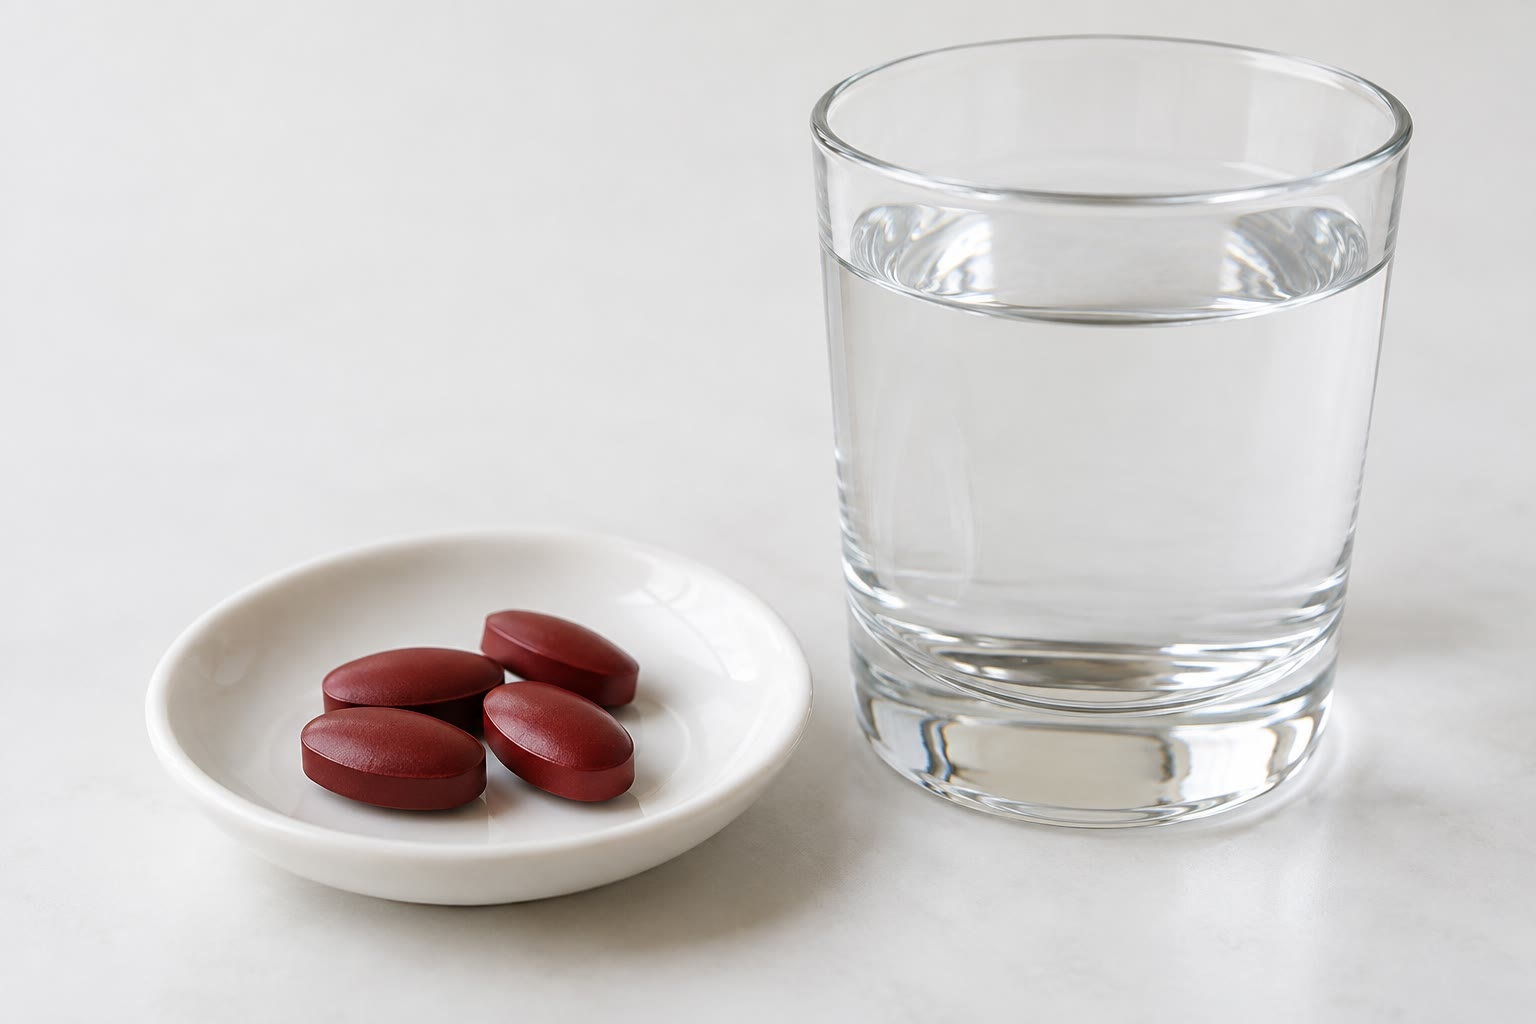
\includegraphics[width=0.45\linewidth]{images/book1/ai/g11-iron-tablets.jpg}

{\small Comprimidos de un suplemento de hierro: ¿cuánto hierro contiene
de verdad cada uno?}
\end{omfigure}

\section{Valorar}

\begin{definition}[Valoración, valorante, disolución valorada]\label{def:g11:titration:titration}
Una \emph{valoración}\index{valoracion@valoración} mide la cantidad de una especie
disuelta haciéndola reaccionar con otra especie cuya concentración se
conoce con precisión. La disolución de concentración conocida, que se
añade desde una bureta, es el \emph{valorante}\index{valorante}; la
disolución que contiene la especie que se quiere medir, colocada en el
matraz, es la \emph{disolución
valorada}\index{disolucion valorada@disolución valorada}.
\end{definition}

\begin{proposition}[Cómo debe ser una reacción de valoración]\label{prop:g11:titration:conditions}
Una reacción se puede usar para una \omterm{def:g11:titration:titration}{valoración} si es total (para que un
\omterm{def:g7:chemical-reactions:reactant}{reactivo} se consuma por completo), rápida (para que cada gota reaccione
enseguida) y única (el \omterm{def:g11:titration:titration}{valorante} no reacciona con nada más en el
matraz).
\end{proposition}

\begin{proof}
Si la reacción se detuviera antes de completarse, fuera por detrás de
las gotas o consumiera \omterm{def:g11:titration:titration}{valorante} en otra cosa, el volumen vertido ya no
mediría la cantidad de la especie valorada.
\end{proof}

\begin{omfigure}
\begin{tikzpicture}[font=\small, scale=0.62]
  \pic[transform shape] at (0,0) {stand={5.8}{1.8}};
  \pic[transform shape] at (1.8,0.68) {stirrer};
  \pic[transform shape] at (1.8,0.68) {erlenmeyer={0.25}{yellow!12}};
  \pic[transform shape] at (1.8,2.98) {burette={0.75}{violet!55}};
  \draw[omProp, thick, <-] (2.15,6.9) -- (4.2,7.4) node[right, text=black,
    align=left] {bureta: valorante\\ (permanganato de potasio)};
  \draw[omProp, thick, <-] (2.55,1.4) -- (4.2,1.9) node[right, text=black,
    align=left] {matraz Erlenmeyer: disolución\\ valorada (hierro(II), ácido)};
  \draw[omProp, thick, <-] (3.0,0.4) -- (4.2,0.3) node[right, text=black]
    {agitador magnético};
\end{tikzpicture}

{\small Un montaje de \omterm{def:g11:titration:titration}{valoración}: la bureta, sujeta a un soporte, vierte
el \omterm{def:g11:titration:titration}{valorante} en la \omterm{def:g11:titration:titration}{disolución valorada}, que se mantiene en agitación.}
\end{omfigure}

\section{La equivalencia}

\begin{definition}[Equivalencia, volumen de equivalencia]\label{def:g11:titration:equivalence}
La \emph{equivalencia}\index{equivalencia} es el momento de una
\omterm{def:g11:titration:titration}{valoración} en que el \omterm{def:g11:titration:titration}{valorante} añadido y la especie valorada están en
las proporciones de la ecuación: los dos se han consumido. El volumen
de \omterm{def:g11:titration:titration}{valorante} vertido en ese momento es el
\emph{volumen de equivalencia}\index{volumen de equivalencia}, $V_E$.
\end{definition}

\begin{proposition}[La relación en la equivalencia]\label{prop:g11:titration:relation}
Para una reacción de \omterm{def:g11:titration:titration}{valoración} $a\,\ce{A} + b\,\ce{B} \longrightarrow$ productos, en la que A (cantidad
$n_A$) se valora con un \omterm{def:g11:titration:titration}{valorante} B de concentración $c_B$, en la
\omterm{def:g11:titration:equivalence}{equivalencia}
\[
  \frac{n_A}{a} = \frac{c_B\, V_E}{b} .
\]
\end{proposition}

\begin{proof}
En la \omterm{def:g11:titration:equivalence}{equivalencia}, la \omterm{def:g6:pure-substances-and-mixtures:mixture}{mezcla} es estequiométrica
(\cref{ch:g10:reaction-progress-table}): A y B, de cantidades iniciales
$n_A$ y $c_B V_E$, se agotan a la vez, así que $n_A / a = c_B V_E / b$.
\end{proof}

\begin{omfigure}
\begin{tikzpicture}
\begin{axis}[width=0.72\linewidth, height=5.6cm, xmin=0, xmax=20,
    ymin=0, ymax=16, xlabel={volumen de valorante añadido (\si{mL})},
    ylabel={cantidad ($\num{e-4}$ \si{mol})}, axis lines*=left, ymajorgrids,
    grid style={gray!20}, tick label style={font=\small},
    label style={font=\small}, legend style={font=\small, at={(0.98,0.97)},
    anchor=north east, draw=none}, legend cell align=left]
  \addplot[very thick, orange!70!black, domain=0:14.3] {14.3 - x};
  \addplot[very thick, violet, domain=14.3:20] {0.2*(x - 14.3)};
  \addplot[very thick, violet, domain=0:14.3, forget plot] {0};
  \legend{\ce{Fe^{2+}} que queda en el matraz, \ce{MnO4^-} en exceso}
  \addplot[dashed, black!60] coordinates {(14.3,0) (14.3,7)};
  \node[font=\small, anchor=west] at (axis cs:14.5,6.5) {$V_E = \qty{14.3}{mL}$};
\end{axis}
\end{tikzpicture}

{\small Hierro(II) valorado con permanganato de \qty{0.0200}{mol/L}: los
\omterm{def:g9:ions:ion}{iones} hierro(II) se agotan exactamente en el \omterm{def:g11:titration:equivalence}{volumen de equivalencia};
después, los \omterm{def:g9:ions:ion}{iones} permanganato ya no se consumen y se acumulan.}
\end{omfigure}

\section{Localizar la equivalencia por un cambio de color}


\begin{proposition}[Ver la equivalencia]\label{prop:g11:titration:colour}
Cuando una de las especies de la \omterm{def:g11:titration:titration}{valoración} tiene color, la \omterm{def:g11:titration:equivalence}{equivalencia}
se ve como un cambio de color del matraz: el color del \omterm{def:g11:titration:titration}{valorante} aparece
y persiste en cuanto el \omterm{def:g11:titration:titration}{valorante} está en exceso, o el color de la
especie valorada desaparece cuando esta se agota.
\end{proposition}

\begin{proof}
Antes de la \omterm{def:g11:titration:equivalence}{equivalencia}, cada \omterm{def:g9:ions:ion}{ion} de \omterm{def:g11:titration:titration}{valorante} que cae en el matraz se
consume enseguida; después de la \omterm{def:g11:titration:equivalence}{equivalencia}, permanece. Por tanto,
una especie coloreada solo está presente en el matraz a un lado de la
\omterm{def:g11:titration:equivalence}{equivalencia}.
\end{proof}

\begin{example}[El permanganato, su propio indicador]\label{ex:g11:titration:permanganate}
El \omterm{def:g9:ions:ion}{ion} permanganato \ce{MnO4^-} es violeta intenso, y los \omterm{def:g9:ions:ion}{iones}
manganeso \ce{Mn^{2+}} que da son casi incoloros; los \omterm{def:g9:ions:ion}{iones} hierro solo
dan a la disolución un tono amarillo pálido. Antes de la \omterm{def:g11:titration:equivalence}{equivalencia},
cada gota violeta se decolora al caer; la primera gota que no se
decolora marca la \omterm{def:g11:titration:equivalence}{equivalencia}: el matraz se vuelve rosa pálido y se
queda así.
\end{example}

\begin{omfigure}
\begin{tikzpicture}[font=\small]
  \pic at (0,0) {erlenmeyer={0.3}{yellow!14}};
  \pic at (3.2,0) {erlenmeyer={0.3}{magenta!10}};
  \pic at (6.4,0) {erlenmeyer={0.3}{violet!45}};
  \node[align=center, anchor=north] at (0,-0.15) {antes de la equivalencia:\\
    amarillo pálido, cada gota\\ se decolora};
  \node[align=center, anchor=north] at (3.2,-0.15) {en la equivalencia:\\
    un rosa tenue que\\ persiste};
  \node[align=center, anchor=north] at (6.4,-0.15) {después de la equivalencia:\\
    violeta (permanganato\\ en exceso)};
\end{tikzpicture}

{\small El matraz de una \omterm{def:g11:titration:titration}{valoración} de hierro(II) con permanganato,
antes de la \omterm{def:g11:titration:equivalence}{equivalencia}, en ella y después. El \omterm{def:g11:titration:equivalence}{volumen de equivalencia}
se lee en el primer rosa que persiste.}
\end{omfigure}

\begin{example}[La vitamina C y el yodo]\label{ex:g11:titration:vitamin-c}
% ledger: aw:C, aw:H, aw:O
La vitamina C, el ácido ascórbico \ce{C6H8O6} ($M = \qty{176.0}{g/mol}$),
es un \omterm{def:g11:redox:oxidant}{reductor}; el yodo \ce{I2} la oxida:
\[
  \ce{C6H8O6 + I2 -> C6H6O6 + 2H+ + 2I-} .
\]
Se valoran \qty{10.0}{mL} de zumo de naranja, con un poco de almidón,
con una disolución de yodo de \qty{5.00e-3}{mol/L}. Antes de la
\omterm{def:g11:titration:equivalence}{equivalencia}, el yodo se consume; la primera gota en exceso vuelve azul
oscuro el almidón. Si $V_E = \qty{5.70}{mL}$, el zumo contenía
$n = \num{5.00e-3} \times \num{5.70e-3} = \qty{2.85e-5}{mol}$ de vitamina
C, es decir, \qty{5.0}{mg} en \qty{10.0}{mL}: \qty{0.50}{g/L}.
\end{example}

\section{Calcular una concentración desconocida}

\begin{method}[Calcular una concentración a partir de una valoración]\label{met:g11:titration:computing}
\begin{enumerate}
  \item Escribir la \omterm{def:g8:balanced-equations:equation}{ecuación ajustada} de la reacción de \omterm{def:g11:titration:titration}{valoración} y leer
        los coeficientes $a$ (especie valorada) y $b$ (\omterm{def:g11:titration:titration}{valorante}).
  \item Leer $V_E$ en la bureta, y calcular la cantidad de \omterm{def:g11:titration:titration}{valorante}
        vertida, $n_B = c_B V_E$.
  \item En la \omterm{def:g11:titration:equivalence}{equivalencia}, $n_A = \dfrac{a}{b}\, c_B V_E$.
  \item Dividir entre el volumen valorado: $c_A = n_A / V_A$. Si la
        muestra se diluyó antes de la \omterm{def:g11:titration:titration}{valoración}, multiplicar por el
        \omterm{def:g10:concentration-and-dilution:dilution}{factor de dilución}.
\end{enumerate}
\end{method}

\begin{example}[Una disolución de hierro(II)]\label{ex:g11:titration:iron}
\qty{20.0}{mL} de una disolución de hierro(II), acidulada, necesitan
$V_E = \qty{12.6}{mL}$ de permanganato de \qty{0.0200}{mol/L}. Aquí
$a = 5$ (\ce{Fe^{2+}}) y $b = 1$ (\ce{MnO4^-}):
$n(\ce{MnO4^-}) = 0.0200 \times 0.0126 = \qty{2.52e-4}{mol}$, así que
$n(\ce{Fe^{2+}}) = 5 \times \num{2.52e-4} = \qty{1.26e-3}{mol}$, y
$c(\ce{Fe^{2+}}) = \num{1.26e-3} / 0.0200 = \qty{0.0630}{mol/L}$.
\end{example}

\section{La valoración como medida}

\begin{inthelab}[Leer una bureta]
La bureta se enjuaga con el \omterm{def:g11:titration:titration}{valorante}, se llena y se libera su punta de
burbujas de \omterm{def:g4:air-a-mixture-of-gases:air}{aire}. El nivel se lee en la parte inferior del menisco, con
el ojo a la misma altura, antes y después de la \omterm{def:g11:titration:titration}{valoración}: el volumen
vertido es la diferencia. Hay una graduación cada \qty{0.1}{mL}, y una
lectura se puede estimar a \qty{0.05}{mL}. Cerca de la \omterm{def:g11:titration:equivalence}{equivalencia}, el
\omterm{def:g11:titration:titration}{valorante} se añade gota a gota, mientras se agita el matraz con la mano
o con el agitador.
\end{inthelab}

\begin{omfigure}
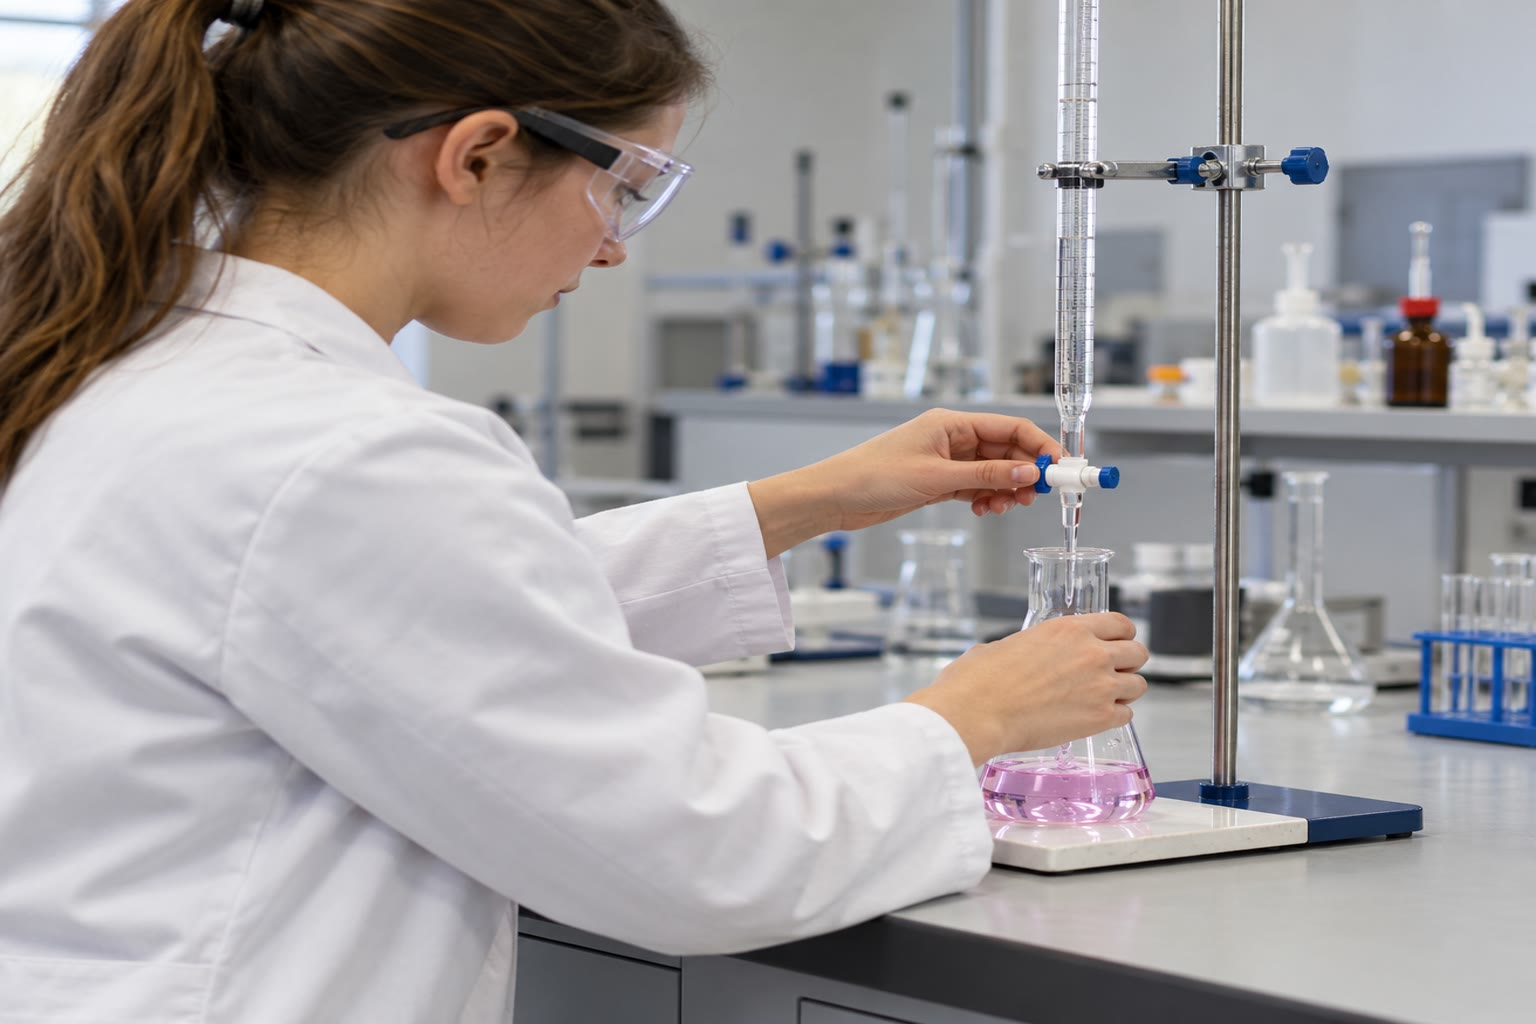
\includegraphics[width=0.48\linewidth]{images/book1/ai/g11-titration-bench.jpg}

{\small Una \omterm{def:g11:titration:titration}{valoración} en curso: bureta, soporte y matraz Erlenmeyer
sobre un azulejo blanco.}
\end{omfigure}

\begin{remark}[¿Qué precisión tiene una valoración?]\label{rem:g11:titration:precision}
Cada lectura de la bureta puede tener un error de unos \qty{0.05}{mL},
y el volumen vertido es la diferencia de dos lecturas: puede tener un
error de hasta \qty{0.1}{mL}. Para $V_E = \qty{14.3}{mL}$, eso es
$0.1 / 14.3 \approx
\qty{0.7}{\percent}$. Un $V_E$ mayor hace más pequeño este error
relativo, y por eso las concentraciones de \omterm{def:g11:titration:titration}{valorante} se eligen de modo
que den volúmenes de \omterm{def:g11:titration:equivalence}{equivalencia} de 10 a \qty{20}{mL} con una bureta de
\qty{25}{mL}. La \omterm{def:g11:titration:titration}{valoración} se repite hasta que dos resultados coinciden
con una diferencia de unos \qty{0.1}{mL}. Un tratamiento más fino de la
incertidumbre de una medida se da en el volumen del primer año
universitario.
\end{remark}

\begin{safety}{\ghs[0.7cm]{GHS03}\ghs[0.7cm]{GHS05}\ghs[0.7cm]{GHS07}\ghs[0.7cm]{GHS08}\ghs[0.7cm]{GHS09}}
% ledger: ghs:KMnO4, ghs:I2
El permanganato de potasio sólido es un \omterm{def:g11:redox:oxidant}{oxidante} que puede avivar un
incendio, corrosivo y nocivo; sus disoluciones diluidas manchan de marrón
la piel y la ropa. Las disoluciones de yodo son nocivas. Gafas y
guantes; los residuos se recogen y nunca se tiran por el fregadero.
\end{safety}

\section{Ejercicios}


\begin{exercise}[$\star$]\label{exo:g11:titration:1}
En una \omterm{def:g11:titration:titration}{valoración}, ¿qué es el \omterm{def:g11:titration:titration}{valorante}? ¿Y la \omterm{def:g11:titration:titration}{disolución valorada}?
¿Qué ocurre en la \omterm{def:g11:titration:equivalence}{equivalencia}?
\end{exercise}

\begin{exercise}[$\star$]\label{exo:g11:titration:2}
¿Qué cantidad de \omterm{def:g9:ions:ion}{iones} permanganato contienen \qty{12.5}{mL} de una
disolución de \qty{0.0200}{mol/L}?
\end{exercise}

\begin{exercise}[$\star$]\label{exo:g11:titration:3}
En la figura de las cantidades en función del volumen vertido, lee el
\omterm{def:g11:titration:equivalence}{volumen de equivalencia}. ¿Qué cantidad de hierro(II) había al principio
en el matraz?
\end{exercise}

\begin{exercise}[$\star$]\label{exo:g11:titration:4}
¿Por qué no hace falta ningún indicador para una \omterm{def:g11:titration:titration}{valoración} con
permanganato?
\end{exercise}

\begin{exercise}[$\star$]\label{exo:g11:titration:5}
En la \omterm{def:g11:titration:equivalence}{equivalencia} de la \omterm{def:g11:titration:titration}{valoración} de hierro(II) con permanganato,
¿cuál es la razón entre la cantidad de hierro(II) y la cantidad de
permanganato vertida? ¿Por qué?
\end{exercise}

\begin{exercise}[$\star\star$]\label{exo:g11:titration:6}
\qty{10.0}{mL} de una disolución acidulada de hierro(II) necesitan
\qty{8.40}{mL} de permanganato de \qty{0.0200}{mol/L}. Calcula la
\omterm{def:g10:concentration-and-dilution:molar-concentration}{concentración molar} de hierro(II) y, después, su \omterm{def:g10:concentration-and-dilution:mass-concentration}{concentración en masa}.
\end{exercise}

\begin{exercise}[$\star\star$]\label{exo:g11:titration:7}
Se \omterm{def:g2:mixing-and-dissolving:dissolve}{disuelve} un comprimido de vitamina C para obtener \qty{100.0}{mL} de
disolución. \qty{10.0}{mL} de ella, con almidón, necesitan
\qty{11.4}{mL} de yodo de \qty{0.0100}{mol/L}. ¿Qué masa de vitamina C
contiene el comprimido?
\end{exercise}

\begin{exercise}[$\star\star$]\label{exo:g11:titration:8}
Una reacción es total, pero tarda varios minutos. ¿Por qué no se puede
usar tal cual para una \omterm{def:g11:titration:titration}{valoración} con cambio de color?
\end{exercise}

\begin{exercise}[$\star\star$]\label{exo:g11:titration:9}
Mira los tres matraces. Una alumna se detiene en un matraz tan violeta
como el tercero. ¿Su \omterm{def:g11:titration:equivalence}{volumen de equivalencia} es demasiado grande o
demasiado pequeño? ¿Qué debería haber hecho cerca de la \omterm{def:g11:titration:equivalence}{equivalencia}?
\end{exercise}

\begin{exercise}[$\star\star$]\label{exo:g11:titration:10}
Una disolución concentrada de hierro(II) se diluye primero diez veces.
Después, \qty{10.0}{mL} de la disolución diluida necesitan
\qty{13.0}{mL} de permanganato de \qty{0.0200}{mol/L}. Halla la
concentración de la disolución concentrada.
\end{exercise}

\begin{exercise}[$\star\star$]\label{exo:g11:titration:11}
% ledger: aw:Fe
La disolución de hierro(II) del ejemplo resuelto del capítulo tiene
$c = \qty{0.0630}{mol/L}$. ¿Qué masa de hierro contiene \qty{1.00}{L} de
ella?
\end{exercise}

\begin{exercise}[$\star\star\star$]\label{exo:g11:titration:12}
Una \omterm{def:g11:titration:titration}{valoración} da $V_E = \qty{7.2}{mL}$. Estima el error relativo debido
a las lecturas de la bureta, y compáralo con el de $V_E = \qty{14.3}{mL}$.
Propón dos maneras de obtener un \omterm{def:g11:titration:equivalence}{volumen de equivalencia} mayor.
\end{exercise}

\begin{exercise}[$\star\star\star$]\label{exo:g11:titration:13}
El peróxido de hidrógeno se valora con permanganato en medio ácido:
\[
  \ce{2MnO4^- + 5H2O2 + 6H+ -> 2Mn^{2+} + 5O2 + 8H2O} .
\]
Un desinfectante se diluye diez veces; \qty{10.0}{mL} de la disolución
diluida necesitan \qty{17.6}{mL} de permanganato de \qty{0.0200}{mol/L}.
Halla la \omterm{def:g10:concentration-and-dilution:molar-concentration}{concentración molar} de peróxido de hidrógeno del desinfectante
y, después, su \omterm{def:g10:concentration-and-dilution:mass-concentration}{concentración en masa} (\ce{H2O2}: \qty{34.0}{g/mol}).
\end{exercise}

\begin{exercise}[$\star\star\star$]\label{exo:g11:titration:14}
Un comprimido de hierro debería contener unos \qty{1.4e-3}{mol} de
hierro(II). ¿Qué concentración de permanganato da un \omterm{def:g11:titration:equivalence}{volumen de
equivalencia} cercano a \qty{15}{mL} con una bureta de \qty{25}{mL}? ¿Qué
fallaría con una disolución diez veces más concentrada?
\end{exercise}

\begin{exercise}[$\star\star\star$]\label{exo:g11:titration:15}
La ecuación de la \omterm{def:g11:titration:titration}{valoración} muestra \ce{8H+} por cada \ce{MnO4^-}. Para
un \omterm{def:g11:titration:equivalence}{volumen de equivalencia} de \qty{14.3}{mL} a \qty{0.0200}{mol/L}, ¿qué
cantidad de \omterm{def:g9:ions:ion}{iones} hidrógeno se consume? ¿Bastan \qty{10}{mL} de un ácido
que contiene \qty{1.0}{mol/L} de \omterm{def:g9:ions:ion}{iones} hidrógeno? ¿Por qué hay que
acidular el matraz?
\end{exercise}

\section{Problema: ¿Es honrado el comprimido de hierro?}

\begin{problem}[{Problema de fin de semana --- un suplemento de hierro
anuncia 80 mg de hierro por comprimido: ¿lo confirma una valoración?}]
\label{pb:g11:titration:1}
% ledger: aw:Fe, aw:S, aw:O, const:NA
La caja de un suplemento de hierro anuncia \qty{80}{mg} de hierro, en
forma de hierro(II), por comprimido. Se tritura un comprimido y se
\omterm{def:g2:mixing-and-dissolving:dissolve}{disuelve} en unos \qty{50}{mL} de ácido sulfúrico diluido; después se
valora con permanganato de potasio de \qty{0.0200}{mol/L}. El rosa tenue
persiste en $V_E = \qty{14.3}{mL}$.

\medskip
\noindent\textbf{Parte I --- La reacción.}
\begin{enumerate}
  \item Nombra los dos \omterm{def:g11:redox:couple}{pares redox} que intervienen. ¿Qué especie es el
        \omterm{def:g11:redox:oxidant}{oxidante} y cuál el \omterm{def:g11:redox:oxidant}{reductor}?
  \item Escribe las dos \omterm{def:g11:redox:couple}{semiecuaciones}.
  \item Combínalas en la ecuación de la \omterm{def:g11:titration:titration}{valoración}, y comprueba que está
        ajustada en carga.
  \item ¿Por qué se \omterm{def:g2:mixing-and-dissolving:dissolve}{disuelve} el comprimido en ácido?
  \item Muestra que la reacción cumple las condiciones de una \omterm{def:g11:titration:titration}{valoración},
        y explica cómo se ve la \omterm{def:g11:titration:equivalence}{equivalencia}.
\end{enumerate}

\medskip
\noindent\textbf{Parte II --- La \omterm{def:g11:titration:titration}{valoración}.}
\begin{enumerate}[resume]
  \item ¿En qué instrumento de vidrio está la disolución de
        permanganato? ¿Cómo se lee su volumen?
  \item ¿De qué color es el matraz antes de la \omterm{def:g11:titration:equivalence}{equivalencia}, y por qué
        pierde el color cada gota?
  \item Calcula la cantidad de permanganato vertida en la \omterm{def:g11:titration:equivalence}{equivalencia}.
\end{enumerate}

\medskip
\noindent\textbf{Parte III --- El hierro.}
\begin{enumerate}[resume]
  \item Deduce la cantidad de hierro(II) del comprimido.
  \item Calcula su masa en miligramos.
  \item Compárala con la etiqueta: ¿diferencia relativa?
  \item El volumen vertido puede tener un error de \qty{0.1}{mL}. ¿En
        cuántos miligramos puede equivocarse la masa de hierro? ¿Queda
        confirmada la etiqueta?
\end{enumerate}

\medskip
\noindent\textbf{Parte IV --- Varios comprimidos.}
\begin{enumerate}[resume]
  \item Otros dos comprimidos dan $V_E = \qty{14.1}{mL}$ y
        \qty{14.4}{mL}. Calcula sus masas de hierro.
  \item Calcula la media de los tres comprimidos.
  \item Los tres resultados difieren en más que el error de la bureta.
        ¿Qué dice esto de los comprimidos?
  \item ¿Habría sido mejor elección un permanganato de
        \qty{0.100}{mol/L}? Explícalo.
  \item Muchos suplementos contienen también vitamina C, un \omterm{def:g11:redox:oxidant}{reductor}.
        ¿Qué efecto tendría en la \omterm{def:g11:titration:titration}{valoración} y en la masa de hierro
        obtenida?
  \item El hierro está presente como sulfato de hierro(II), \ce{FeSO4}.
        ¿Qué masa de él contiene un comprimido?
  \item ¿Cuántos \omterm{def:g9:ions:ion}{iones} hierro(II) son?
  \item Da la respuesta final: ¿qué masa de hierro contiene un
        comprimido?
\end{enumerate}
\end{problem}
